\section{Qatar Grand Prix}

\subsection{Circuit Analysis}

\textbf{Circuit Name:} Losail International Circuit (Lusail, Qatar) \\
\textbf{Length:} 5.419 km - \textbf{Laps:} 57 - \textbf{Total Distance:} 308.611 km

\begin{figure}[H]
    \centering
    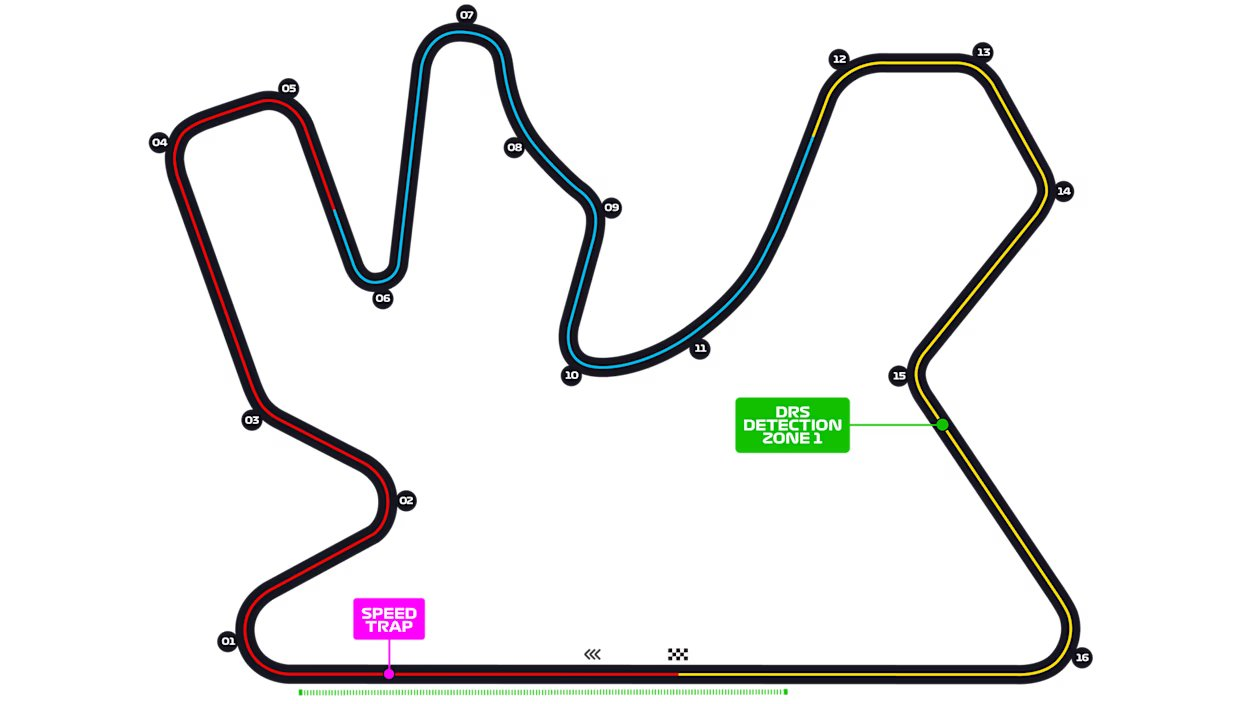
\includegraphics[width=0.75\linewidth]{images/23.Qatar_Circuit.jpg}
\end{figure}

\begin{itemize}
    \item \textbf{Lap Record} : 1:20.827 (2021, Lewis Hamilton - Mercedes).

    \item \textbf{Number of Corners \& Key Features} : 16 turns (10 right, 6 left). \\
    Fast, flowing track with medium–high downforce demand. Long straights combined with technical sequences.
    
    \item \textbf{Braking Zones \& Traction} : Main braking into Turn 1. \\
    High-speed corners put stress on front tyres, with traction key in final sector.

    \item \textbf{DRS \& Overtaking} : One long DRS zone on the main straight. \\
    Overtaking possible in Turn 1, otherwise difficult due to narrow track.

    \item \textbf{Tyre Degradation \& Strategy} : Hot conditions typically strain tyres, but night race reduces temperatures. \\
    Still, abrasive surface leads to high wear: multi-stop strategies usual.

    \item \textbf{Weather \& Environment} : Night race under floodlights. \\
    Air temperature cooler but track remains abrasive and dusty, reducing grip.
\end{itemize}

\textbf{Strategic Summary :} Lusail rewards aerodynamic balance and tyre preservation. Track evolution significant, safety cars often influence strategy.

\subsection{Race Analysis}

\textbf{Date:} Sprint : 30 November 2024 - 17:00 local time\\
Race : 1 December 2024 — 19:00 local time 

\begin{itemize}
    \item \textbf{Sprint Qualifying:} \textbf{Pole Position:} Lando Norris (McLaren) - 1:21.012.\\
    Grid : Russell 2nd, Piastri 3rd, Sainz 4th.

    \item \textbf{Sprint Summary} : \textbf{Winner:} Oscar Piastri (McLaren). \\
    \textbf{Podium}: 1. Piastri - 2. Norris - 3. Russell. \\
    Norris slowed deliberately at the end to give Piastri the win in return for São Paulo. Haas scored big with Hülkenberg P7. Verstappen only 8th. McLaren strengthened constructors’ lead.

    \item \textbf{Qualifying Summary} : \textbf{Fastest Lap in Q3:} Max Verstappen (Red Bull) – 1:20.520. \\
    \textbf{Pole Position:} George Russell (Mercedes) – 1:20.575 (new track record). \\
    Grid: Verstappen 2nd, Norris 3rd, Piastri 4th, Leclerc 5th. \\
    Max Verstappen, who finished 1st during the qualifications, was penalised of on grid place for impeding.

    \item \textbf{Race Summary} : \textbf{Winner:} Max Verstappen (Red Bull). \\
    \textbf{Podium:} 1. Verstappen - 2. Leclerc - 3. Piastri. \\
    Norris dropped to P10 after 10s stop-and-go penalty under double yellow, but claimed fastest lap. \\
    Zhou scored Kick Sauber’s first points of the season (P8). \\
    \textbf{Multiple incidents}: Ocon and Colapinto out at start, Stroll–Albon clash, Pérez retired with clutch issues, Hülkenberg crashed out lap 39.

    \item \textbf{Strategies} : \\
    - Red Bull: Verstappen flawless, benefitted from Safety Car pit stop. Pérez retired. \\
    - Ferrari: Leclerc solid P2, Sainz P6. \\
    - McLaren: Piastri strong P3, Norris sabotaged by penalty but fastest lap. \\
    - Mercedes: Russell P4 despite penalty, Hamilton only P12 after drive-through. \\
    - Alpine: Gasly excellent P5, Ocon retired at start. \\
    - Kick Sauber: Zhou P8, first points in 2024. 

    \item \textbf{Performance Trends} : \textbf{Red Bull} back on form with Verstappen dominant.\\
    \textbf{Ferrari} consistent, Leclerc under pressure from Piastri. \\
    \textbf{McLaren} still competitive but less dominant. \\
    \textbf{Mercedes} strong in quali but inconsistent in race.\\
    \textbf{Alpine} revived thanks to Gasly. \\
    \textbf{Kick Sauber} celebrated breakthrough points.

    \item \textbf{Championship Impact} : \\
    \textbf{Drivers:} Verstappen 429 pts (Champion), Norris 349, Leclerc 341. \\
    \textbf{Constructors:} McLaren 640, Ferrari 619, Red Bull 581, Mercedes 446. \\
    Abu Dhabi will decide Constructors’ title between McLaren and Ferrari.
\end{itemize}

\textbf{Key Takeaway :} Verstappen dominated under the lights of Lusail. Gasly starred for Alpine, Zhou delivered Kick Sauber’s long-awaited points, and penalties shaped Norris’ and Hamilton’s races. The championship finale at Abu Dhabi is set up for a McLaren vs Ferrari showdown.

\subsection{Link \& Takeaway}

\begin{itemize}
    \item Verstappen proved Red Bull still has sharp teeth, dominating despite title already secured. 
    \item Ferrari stayed in the fight: Leclerc maximised podium points. 
    \item McLaren’s teamwork in the Sprint contrasted with Norris’ penalty in the GP. 
    \item Alpine and Gasly shone, Kick Sauber finally off the mark thanks to Zhou. 
    \item The Constructors’ title will be decided in Abu Dhabi, 21 points between McLaren and Ferrari. 
\end{itemize}
